\documentclass[11pt,aspectratio=169]{beamer}

% Explicative slide deck for the Part I compact analytical model.
% Companion source of truth: intergenerational_housing_fertility_part1.tex
% Design rule: one idea per frame, words before math, pictures where they explain.

\usepackage[T1]{fontenc}
\usepackage{lmodern}
\usepackage{amsmath,amssymb,mathtools}
\usepackage{booktabs}
\usepackage{tikz}
\usetikzlibrary{arrows.meta,positioning,calc,decorations.pathreplacing}
\usepackage{appendixnumberbeamer}

\setbeamertemplate{navigation symbols}{}
\setbeamertemplate{itemize items}[circle]
\setbeamertemplate{itemize subitem}{--}
\setbeamertemplate{footline}[frame number]
\setbeamersize{text margin left=0.85cm,text margin right=0.85cm}

\definecolor{accent}{RGB}{38,98,135}
\definecolor{gapred}{RGB}{160,52,42}
\definecolor{okgreen}{RGB}{44,110,73}
\definecolor{softblue}{RGB}{231,242,248}
\definecolor{softgreen}{RGB}{232,244,236}
\definecolor{softred}{RGB}{249,235,232}
\definecolor{softgrey}{RGB}{242,242,242}

\setbeamercolor{frametitle}{fg=accent}
\setbeamerfont{frametitle}{series=\bfseries,size=\large}
\setbeamercolor{title}{fg=accent}
\setbeamercolor{alerted text}{fg=gapred}
\setbeamercolor{block title}{fg=black,bg=softblue}
\setbeamercolor{block body}{fg=black,bg=softblue!45}
\setbeamercolor{block title example}{fg=black,bg=softgreen}
\setbeamercolor{block body example}{fg=black,bg=softgreen!45}
\setbeamercolor{block title alerted}{fg=black,bg=softred}
\setbeamercolor{block body alerted}{fg=black,bg=softred!45}
\linespread{1.1}

\newcommand{\dd}{\mathrm d}
\newcommand{\1}{\mathbf 1}
\newcommand{\HH}{\mathcal H}
\newcommand{\Mbar}{\bar M}

\tikzset{
  ebox/.style={draw=black!70,rounded corners=2pt,thick,align=center,inner sep=5pt,fill=white,font=\footnotesize},
  bluee/.style={ebox,fill=softblue},
  greene/.style={ebox,fill=softgreen},
  rede/.style={ebox,fill=softred},
  greye/.style={ebox,fill=softgrey,draw=black!45,text=black!70},
  flow/.style={-{Latex[length=2.6mm]},thick,draw=accent},
  greyflow/.style={-{Latex[length=2.6mm]},thick,draw=black!45},
  redflow/.style={-{Latex[length=2.6mm]},thick,draw=gapred},
  lab/.style={font=\scriptsize,text=black!75,align=center},
  axisline/.style={->,thick,draw=black!75}
}

\title{Intergenerational Housing Allocation and Fertility}
\subtitle{Part I: Compact Analytical Model}
\author{Tommaso De Santo}
\date{June 2026}

\begin{document}

% ============================================================
\begin{frame}
\titlepage
\vspace{-1.2em}
\begin{center}
\small
\textit{When does limited access to family-capable housing reduce fertility,\\ and which policies actually relax that limit?}
\end{center}
\end{frame}

% ============================================================
\begin{frame}{The argument in one slide}
\small
\begin{enumerate}\setlength{\itemsep}{0.4em}
  \item \textbf{Children require space, not just goods.} Each child claims $\kappa$ units of housing services and $\chi_i$ goods; parents consume what remains of the house and the budget.
  \item \textbf{Family-sized space is rationed.} Rental menus stop at $\bar h^R$; buying requires a down payment and payment capacity. For each household, all of these frictions collapse into \alert{one number}: the effective family-housing cap $H_i^m$.
  \item \textbf{A binding cap makes children more expensive.} The shadow price of a child is $\chi_i+\kappa(q^m+\zeta_i^m)$: space for the child is priced at the household's \emph{own} shadow value of space, which exceeds the market price by the access gap $\zeta_i^m$.
  \item \textbf{This yields a policy test.} Fertility responds only if the policy relaxes the \emph{binding} component of $H_i^m$. The local effect is exposure $\times$ pass-through $\times$ fertility response, plus an entry margin.
\end{enumerate}
\smallskip
\begin{exampleblock}{}
\centering
One statistic does two jobs: under equal scaling $\Psi_i^m\propto\zeta_i^m$ --- the gap that measures misallocation is the gap that predicts births.
\end{exampleblock}
\end{frame}

% ============================================================
\begin{frame}{The economy in one picture}
\begin{center}
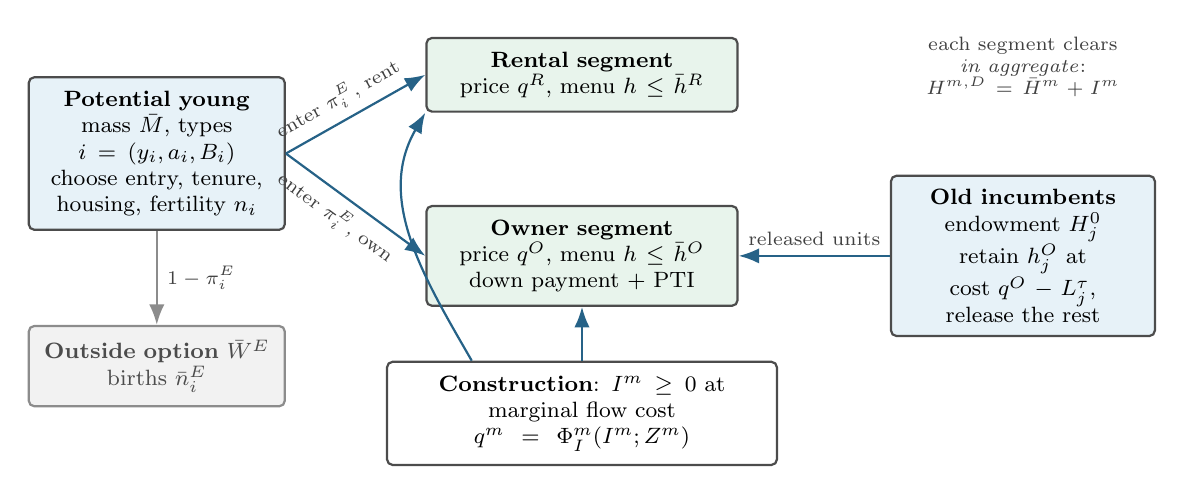
\begin{tikzpicture}[x=1cm,y=1cm]
  % young side
  \node[bluee,text width=2.9cm] (young) at (0,2.3) {\textbf{Potential young}\\ mass $\Mbar$, types $i=(y_i,a_i,B_i)$\\ choose entry, tenure,\\ housing, fertility $n_i$};
  \node[greye,text width=2.9cm] (out) at (0,-0.4) {\textbf{Outside option} $\bar W^E$\\ births $\bar n_i^E$};
  \draw[greyflow] (young) -- (out) node[midway,right,lab]{$1-\pi_i^E$};

  % segments
  \node[greene,text width=3.6cm] (rent) at (5.4,3.3) {\textbf{Rental segment}\\ price $q^R$, menu $h\le\bar h^R$};
  \node[greene,text width=3.6cm] (own) at (5.4,1.0) {\textbf{Owner segment}\\ price $q^O$, menu $h\le\bar h^O$\\ down payment $+$ PTI};
  \draw[flow] (young.east) -- (rent.west) node[pos=0.45,above,sloped,lab]{enter $\pi_i^E$, rent};
  \draw[flow] (young.east) -- (own.west) node[pos=0.45,below,sloped,lab]{enter $\pi_i^E$, own};

  % old side
  \node[bluee,text width=3.0cm] (old) at (11.0,1.0) {\textbf{Old incumbents}\\ endowment $H_j^0$\\ retain $h_j^O$ at cost $q^O-L_j^\tau$,\\ release the rest};
  \draw[flow] (old.west) -- (own.east) node[midway,above,lab]{released units};

  % construction
  \node[ebox,text width=4.6cm] (con) at (5.4,-1.0) {\textbf{Construction}: $I^m\ge0$ at\\ marginal flow cost $q^m=\Phi_I^m(I^m;Z^m)$};
  \draw[flow] (con.north) -- (own.south);
  \draw[flow] ($(con.north)+(-1.4,0)$) to[out=120,in=240] (rent.south west);

  % clearing note
  \node[lab,text width=3.0cm] at (11.0,3.4) {each segment clears\\ \emph{in aggregate}:\\ $H^{m,D}=\bar H^m+I^m$};
\end{tikzpicture}
\end{center}
\vspace{0.2em}
\footnotesize
No pairwise matching of old units to young buyers: $(q^R,q^O)$ clear two aggregate markets. The asset price $P^O=q^O/\rho_p$ matters only for down payments.
\end{frame}

% ============================================================
\begin{frame}{Children require goods \emph{and} space}
\small
Each child claims $\chi_i$ goods and $\kappa$ units of housing services. Parents consume the residual:
\[
c_i=C_i-\chi_i n_i,
\qquad
s_i=h_i-\kappa n_i,
\qquad
u_i^Y=\log c_i+\alpha\log s_i+\beta\log n_i .
\]
\begin{itemize}\setlength{\itemsep}{0.4em}
  \item Same house, one more child $\Rightarrow$ less adult space $s_i$. Same budget, one more child $\Rightarrow$ less adult consumption $c_i$. \textbf{Children compete with their parents for space} --- this is the engine of the model.
  \item Substituting $h=s+\kappa n$ into a branch budget $c+q^m h+\chi_i n=y_i$ gives
  \[
  c_i+q^m s_i+\underbrace{(\chi_i+\kappa q^m)}_{\text{full price of a child}} n_i = y_i .
  \]
  Unconstrained, a child costs its goods plus the space it occupies, at the \emph{market} price of space.
  \item Because $\beta\log n_i$ rules out $n_i=0$, every entrant has positive completed fertility: the model is about the \textbf{intensive margin}, not childlessness.
\end{itemize}
\end{frame}

% ============================================================
\begin{frame}{Family-sized space lives in the owner segment}
\small
\textbf{Two segments, two menus.} Renting and owning offer different size menus:
\[
\HH^R=\{h:0<h\le\bar h^R\},
\qquad
\HH^O=\{h:0<h\le\bar h^O\},
\qquad
\bar h^R<\bar h^O .
\]
Large family-sized units exist mainly in the owner segment. The caps are individual occupancy menus, not aggregate stocks.

\medskip
\textbf{Supply.} Each segment has inherited stock plus net construction, supplied at increasing marginal cost:
\[
H^m=\bar H^m+I^m,
\qquad
q^m=\Phi_I^m(I^m;Z^m)
\quad\text{(flow units).}
\]

\medskip
\textbf{Buying needs finance.} Owners face the asset price
\[
P^O=\frac{q^O}{r+\delta^O+\tau^p},
\]
which enters \emph{only} the down-payment constraint. Note for later: a higher property tax $\tau^p$ \emph{lowers} $P^O$, hence lowers the required down payment.
\end{frame}

% ============================================================
\begin{frame}{Each household's frictions collapse into one cap}
\small
Conditional on entry, household $i$ solves a renter branch and an owner branch and picks the better one, $W_i^Y=\max\{W_i^R,W_i^O\}$. In each branch, everything that limits family space is one number:
\[
H_i^R=\bar h^R,
\qquad
H_i^O=\min\Big\{
\underbrace{\bar h^O}_{\text{menu}},\;
\underbrace{\tfrac{A_i(x)\,\rho_p}{(1-\phi)\,q^O}}_{\text{down payment}},\;
\underbrace{\tfrac{\psi y_i}{q^O}}_{\text{payment-to-income}}
\Big\},
\qquad \rho_p=r+\delta^O+\tau^p .
\]
\begin{columns}[T]
\begin{column}{0.52\textwidth}
\begin{center}
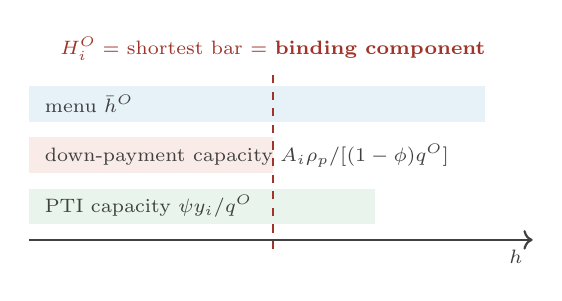
\begin{tikzpicture}[x=1cm,y=1cm]
  \draw[axisline] (0,0) -- (6.4,0) node[below left,lab]{$h$};
  % menu bar
  \fill[softblue]  (0,1.50) rectangle (5.8,1.95); \node[lab,anchor=west] at (0.08,1.725){menu $\bar h^O$};
  \fill[softred]   (0,0.85) rectangle (3.1,1.30); \node[lab,anchor=west] at (0.08,1.075){down-payment capacity $A_i\rho_p/[(1-\phi)q^O]$};
  \fill[softgreen] (0,0.20) rectangle (4.4,0.65); \node[lab,anchor=west] at (0.08,0.425){PTI capacity $\psi y_i/q^O$};
  \draw[dashed,thick,gapred] (3.1,-0.12) -- (3.1,2.15) node[above,lab,text=gapred]{$H_i^O=$ shortest bar $=$ \textbf{binding component}};
\end{tikzpicture}
\end{center}
\end{column}
\begin{column}{0.44\textwidth}
\footnotesize
Wealth is \textbf{pledgeable only}:
\[
A_i(x)=a_i+xB_i+T_i^b(x),\quad x=1-\tau^b .
\]
It backs the down payment but is not spendable in the flow budget. So inheritances and the estate tax work through \emph{owner access}, not through consumption.
\end{column}
\end{columns}
\medskip
\alert{$H_i^m$ is the only object a policy can usefully move in this model.}
\end{frame}

% ============================================================
\begin{frame}{A binding cap shows up as an access gap $\zeta$}
\small
When the cap binds, the household values space above its market price. The branch first-order conditions give
\[
\frac{u_{h}}{u_{c}}
=\frac{\alpha c_i^m}{s_i^m}
= q^m+\zeta_i^m,
\qquad
\zeta_i^m\ge0,
\]
where $\zeta_i^m$ is the \textbf{goods value of one more unit of space} --- zero when unconstrained. For owners it decomposes as
\[
\zeta_i^O
=
\underbrace{\frac{\mu_i}{\lambda_i^O}(1-\phi)P^O+\frac{\eta_i}{\lambda_i^O}q^O}_{\zeta_i^{O,F}:\ \text{financial (DP, PTI)}}
+
\underbrace{\frac{\theta_i^O}{\lambda_i^O}}_{\text{menu}} .
\]
\begin{block}{Why this matters for fertility (Proposition 1)}
\centering
$\displaystyle
\frac{\beta c_i^m}{n_i^m}
=
\chi_i+\kappa\big(q^m+\zeta_i^m\big)
$
\smallskip

A child's space requirement is priced at the household's \emph{own} shadow value of space:\\
children get more expensive even at unchanged market prices. $\zeta_i^m$ is the model's\\
misallocation thermometer --- it returns in the efficiency result \emph{and} in the policy formula.
\end{block}
\end{frame}

% ============================================================
\begin{frame}{Space caps are fertility caps}
\begin{columns}[T]
\begin{column}{0.50\textwidth}
\begin{center}
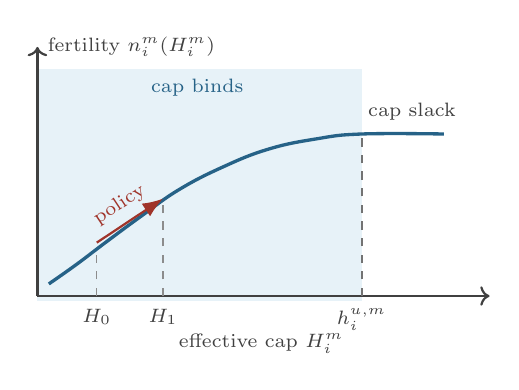
\begin{tikzpicture}[x=0.58cm,y=0.57cm]
  \fill[softblue] (0.7,0.45) rectangle (7.8,5.6);
  \node[lab,text=accent] at (4.2,5.2) {cap binds};
  \draw[axisline] (0.7,0.55) -- (10.6,0.55);
  \node[lab] at (5.6,-0.5) {effective cap $H_i^m$};
  \draw[axisline] (0.7,0.55) -- (0.7,6.1) node[right,lab]{fertility $n_i^m(H_i^m)$};
  \draw[very thick,draw=accent]
    plot[smooth,tension=0.72] coordinates {
      (0.95,0.82) (1.55,1.25) (2.2,1.75) (3.0,2.35)
      (3.8,2.92) (4.75,3.42) (5.75,3.82) (6.8,4.05)
      (7.8,4.16) (9.6,4.16)
    };
  \draw[dashed,thick,draw=black!55] (7.8,0.55) -- (7.8,4.16);
  \node[lab,below] at (7.8,0.48) {$h_i^{u,m}$};
  \node[lab,above] at (8.9,4.25) {cap slack};
  \draw[dashed,draw=black!45] (2.0,0.55) -- (2.0,1.62);
  \node[lab,below] at (2.0,0.48) {$H_0$};
  \draw[dashed,draw=black!45] (3.45,0.55) -- (3.45,2.7);
  \node[lab,below] at (3.45,0.48) {$H_1$};
  \draw[redflow] (2.0,1.74) -- (3.45,2.72) node[midway,above,sloped,lab,text=gapred]{policy};
\end{tikzpicture}
\end{center}
\end{column}
\begin{column}{0.47\textwidth}
\small
With a binding cap, $h=H$ and fertility solves
\[
\frac{\beta}{n}=\frac{\chi}{c(H)}+\frac{\alpha\kappa}{s(H)} .
\]
Implicit differentiation:
\[
\frac{\dd n}{\dd H}
=
\frac{\dfrac{\alpha\kappa}{s^2}-\dfrac{\chi q}{c^2}}
{\dfrac{\beta}{n^2}+\dfrac{\chi^2}{c^2}+\dfrac{\alpha\kappa^2}{s^2}} .
\]
\footnotesize
Two forces: more space lowers the \emph{crowding cost} of a child (numerator term $\alpha\kappa/s^2$), but the household also buys more housing at $q$, squeezing consumption ($\chi q/c^2$). The curve is within one tenure branch; each branch has its own curve.
\end{column}
\end{columns}
\end{frame}

% ============================================================
\begin{frame}{When does more space mean more children?}
\small
\begin{block}{Sign condition (exact, branch by branch)}
Relaxing a strictly binding cap raises fertility at \emph{every} binding cap level if and only if
\[
\chi_i\;\le\;\frac{\kappa q^m}{\alpha},
\]
i.e.\ the child input bundle is \textbf{not more consumption-intensive} than the adult residual bundle.
\end{block}
\medskip
\begin{itemize}\setlength{\itemsep}{0.45em}
  \item Read $\kappa q^m/\chi_i\ge\alpha$: the child's housing-to-goods expenditure ratio is at least the adult's. Children are, if anything, \emph{space-intensive} --- the empirically natural case.
  \item \textbf{Benchmark: equal scaling} $\chi_i=\kappa q^m/\alpha$. A child is then a scaled copy of the adult bundle, and any relaxation of a strictly binding cap raises fertility until the cap stops binding.
  \item If instead $\chi_i>\kappa q^m/\alpha$ (goods-hungry children), fertility can \emph{fall} when the cap is relaxed near the unconstrained optimum: the extra housing purchase squeezes consumption, and consumption is what goods-hungry children need most.
\end{itemize}
\end{frame}

% ============================================================
\begin{frame}{One gap, two jobs: $\Psi_i^m\propto\zeta_i^m$}
\small
Define the within-branch fertility response $\Psi_i^m=\partial n_i^m/\partial H_i^m$ at a binding cap.

\begin{exampleblock}{Corollary (equal scaling)}
\[
\Psi_i^m
=
\frac{\kappa}{\alpha}\,
\frac{\zeta_i^m}{c_i^m}\,
\Omega_i^m,
\qquad
\Omega_i^m=
\frac{\dfrac{\alpha}{s_i^m}+\dfrac{q^m}{c_i^m}}
{\dfrac{\beta}{(n_i^m)^2}+\dfrac{\chi_i^2}{(c_i^m)^2}+\dfrac{\alpha\kappa^2}{(s_i^m)^2}}
>0 .
\]
\end{exampleblock}

\begin{itemize}\setlength{\itemsep}{0.45em}
  \item $\Psi_i^m>0$ \emph{iff} $\zeta_i^m>0$: fertility responds exactly for the households whose access constraint bites, and more for those where it bites harder.
  \item The entry margin runs on the same object: relaxing the cap raises the inside value by $\Theta_i^m=\lambda_i^m\zeta_i^m=\zeta_i^m/c_i^m$ utils per unit.
  \item So \textbf{both} margins of the policy formula scale with the access gap per unit of adult consumption, $\zeta_i^m/c_i^m$ --- the misallocation measure \emph{is} the fertility lever.
\end{itemize}
\end{frame}

% ============================================================
\begin{frame}{The old side: retention can be tax-subsidized}
\small
Old incumbents enter with owner housing $H_j^0$ and choose how much to retain:
\[
\max_{c,h,e}\;\log c+\gamma\log h+\mathcal B_j(e)
\quad\text{s.t.}\quad
c+e+\big(q^O-L_j^\tau\big)h=m_j+q^O H_j^0,
\qquad 0\le h\le H_j^0 .
\]
\begin{itemize}\setlength{\itemsep}{0.45em}
  \item \textbf{Assessment lock-in:} $L_j^\tau=\tau^pP^O-\tilde\tau_j\tilde P_j\ge0$ is the gap between the market property-tax cost and the protected assessed cost. Keeping the unit is artificially cheap; releasing it forfeits the protection.
  \item Interior retention satisfies $MV_j^O=q^O-L_j^\tau$: the old hold space past the point where their true valuation matches its social cost. $L_j^\tau$ is \alert{a subsidy to sitting, not a preference}.
  \item Bequests are a true preference margin ($\mathcal B_j'=1/c_j^O$), not a distortion. The planner counts old housing utility and warm glow --- old occupancy is \emph{not} inefficient by itself.
\end{itemize}
\medskip
\begin{block}{}
\centering
The young-access mechanism does not need this: it stands even at $L_j^\tau=0$.\\ Lock-in is an optional \emph{amplifier} of family-space scarcity.
\end{block}
\end{frame}

% ============================================================
\begin{frame}{Equilibrium: markets clear --- clearing is not efficiency}
\small
A competitive equilibrium: prices $(q^R,q^O)$, asset price $P^O$, construction $(I^R,I^O)$ such that
\begin{itemize}\setlength{\itemsep}{0.3em}
  \item young households solve both branches, pick tenure, enter with logit probability $\pi_i^E$;
  \item old households solve the retention problem; builders set $q^m=\Phi_I^m$;
  \item both segments clear \emph{in aggregate}:
  \[
  \Mbar\!\int\!\pi_i^E\1\{o_i{=}R\}h_i\,\dd G_Y=\bar H^R+I^R,
  \qquad
  \Mbar\!\int\!\pi_i^E\1\{o_i{=}O\}h_i\,\dd G_Y+\!\int\! h_j^O\,\dd F_O=\bar H^O+I^O;
  \]
  \item housing payments are transfers, closed by lump-sum rebates; only construction uses real resources.
\end{itemize}
\medskip
\begin{alertblock}{The punchline}
Both segments can clear while the \emph{marginal unit of owner space} is held by the wrong hands: financially constrained young value it at $q^O+\zeta_i^{O,F}$ and cannot buy more; tax-protected old hold it at $q^O-L_j^\tau$. Prices equate aggregates, not marginal values across people.
\end{alertblock}
\end{frame}

% ============================================================
\begin{frame}{Two gaps separate the equilibrium from the planner}
\footnotesize
Planner: same preferences, same menus, same construction technology. Financial (DP/PTI) constraints are \emph{implementation} constraints the planner can relax with financing instruments at zero marginal resource cost. Fertility-neutral ($\nu_i^g=0$), conditional on entry measure and tenure assignments.
\begin{center}
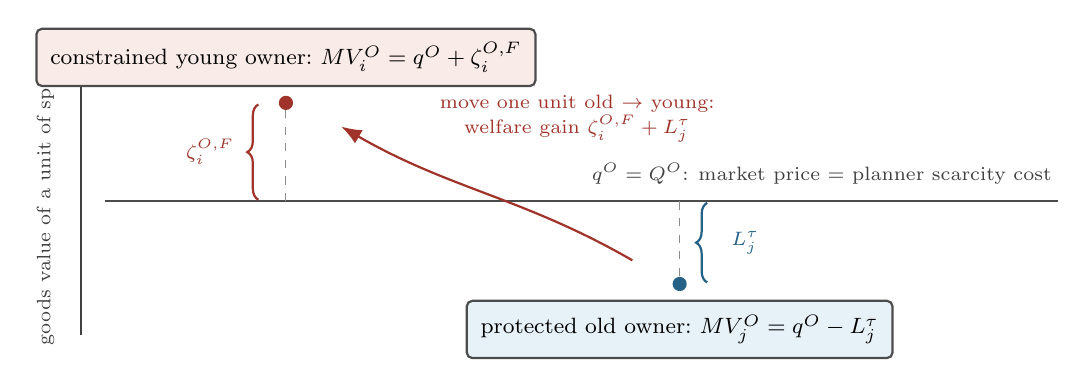
\begin{tikzpicture}[x=1cm,y=1cm]
  % axis
  \draw[axisline] (0,-1.7) -- (0,1.6);
  \node[lab,rotate=90,anchor=south] at (-0.22,0) {goods value of a unit of space};
  % market line
  \draw[thick,black!70] (0.3,0) -- (12.4,0);
  \node[lab,anchor=south east] at (12.45,0.09) {$q^O=Q^O$: market price $=$ planner scarcity cost};
  % young dot
  \fill[gapred] (2.6,1.25) circle (0.09);
  \node[ebox,fill=softred,anchor=south] at (2.6,1.45) {constrained young owner:\ $MV_i^O=q^O+\zeta_i^{O,F}$};
  \draw[decorate,decoration={brace,amplitude=4pt},thick,gapred] (2.25,0.02) -- (2.25,1.23) node[midway,left=5pt,lab,text=gapred]{$\zeta_i^{O,F}$};
  \draw[black!45,dashed] (2.6,0) -- (2.6,1.25);
  % old dot
  \fill[accent] (7.6,-1.05) circle (0.09);
  \node[ebox,fill=softblue,anchor=north] at (7.6,-1.25) {protected old owner:\ $MV_j^O=q^O-L_j^\tau$};
  \draw[decorate,decoration={brace,amplitude=4pt},thick,accent] (7.95,-1.03) -- (7.95,-0.02) node[midway,right=5pt,lab,text=accent]{$L_j^\tau$};
  \draw[black!45,dashed] (7.6,0) -- (7.6,-1.05);
  % transfer arrow
  \draw[redflow] (7.0,-0.75) to[out=150,in=-30] (3.3,0.95);
  \node[lab,text=gapred] at (6.3,1.05) {move one unit old $\to$ young:\\ welfare gain $\zeta_i^{O,F}+L_j^\tau$};
\end{tikzpicture}
\end{center}
\vspace{0.1em}
The equilibrium satisfies the planner's marginal conditions \textbf{only if} $\zeta_i^{O,F}=0$ and $L_j^\tau=0$. Binding \emph{menus} are not a gap (the planner faces the same menus); entry and tenure-assignment margins are not characterized.
\end{frame}

% ============================================================
\begin{frame}{A policy test: does it relax the binding constraint?}
\begin{center}
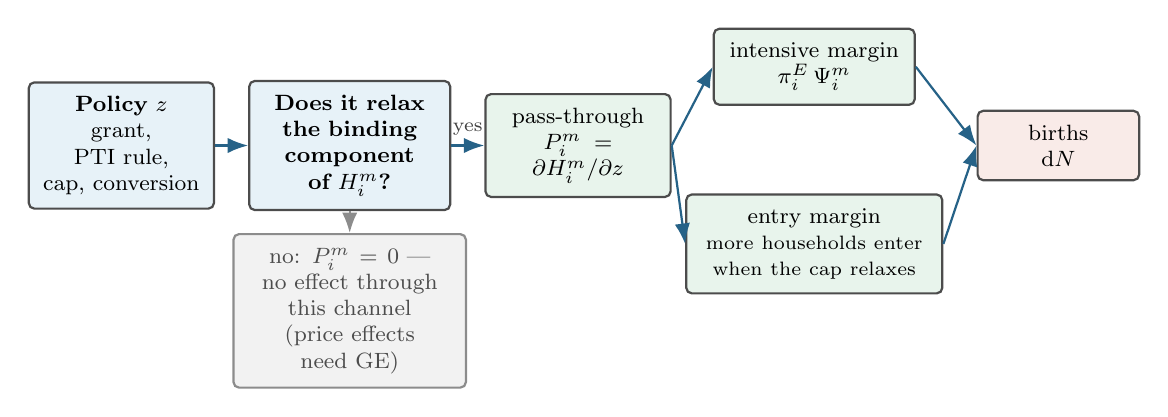
\begin{tikzpicture}[x=1cm,y=1cm]
  \node[bluee,text width=2.0cm] (pol) at (0,0)    {\textbf{Policy $z$}\\ grant, PTI rule,\\ cap, conversion};
  \node[bluee,text width=2.2cm] (gate) at (2.9,0) {\textbf{Does it relax the binding component of $H_i^m$?}};
  \node[greene,text width=2.0cm] (pass) at (5.8,0){pass-through\\ $P_i^m=\partial H_i^m/\partial z$};
  \node[greene,text width=2.2cm] (psi) at (8.8,1.0){intensive margin\\ $\pi_i^E\,\Psi_i^m$};
  \node[greene,text width=2.9cm] (ent) at (8.8,-1.25){entry margin\\ {\scriptsize more households enter when the cap relaxes}};
  \node[rede,text width=1.7cm] (dn) at (11.9,0)   {births\\ $\dd N$};
  \node[greye,text width=2.6cm] (no) at (2.9,-2.1){no: $P_i^m=0$ --- no effect through this channel\\ (price effects need GE)};
  \draw[flow] (pol) -- (gate);
  \draw[flow] (gate) -- (pass) node[midway,above,lab]{yes};
  \draw[greyflow] (gate) -- (no);
  \draw[flow] (pass.east) -- (psi.west);
  \draw[flow] (pass.east) -- (ent.west);
  \draw[flow] (psi.east) -- (dn.west);
  \draw[flow] (ent.east) -- (dn.west);
\end{tikzpicture}
\end{center}
\small
The cap is a \emph{minimum} of three components. A policy that improves a slack component does nothing here: a cheaper small apartment does not relax a binding down-payment constraint, and a down-payment grant does nothing for a renter capped by the rental menu.
\end{frame}

% ============================================================
\begin{frame}{The local policy decomposition}
\small
Holding prices, tenure choices, and active sets fixed ($\mathcal B_m$ = entrant types whose cap binds in branch $m$):
{\footnotesize
\[
\left.\frac{\dd N}{\dd z}\right|_{q,o,\mathcal A}
=
\Mbar\sum_{m\in\{R,O\}}\int_{\mathcal B_m}
\Bigg[
\underbrace{\pi_i^E\,\Psi_i^m}_{\substack{\text{intensive: entered mass}\\ \times\ \text{fertility response}}}
+
\underbrace{(n_i^m-\bar n_i^E)\,\frac{\pi_i^E(1-\pi_i^E)}{\kappa_E}\,\Theta_i^m}_{\substack{\text{entry: births per entrant}\\ \times\ \text{sensitivity}\ \times\ \text{value of relaxation}}}
\Bigg]
\underbrace{P_i^m(z)}_{\substack{\text{pass-through}\\ \text{to the cap}}}
\,\dd G_Y(i)
\]}
\medskip
\textbf{Read it as:} exposure $\times$ pass-through $\times$ response, plus entry. Births count relative to outside-option fertility $\bar n_i^E$ (zero under the baseline normalization).

\medskip
\begin{alertblock}{What this formula deliberately leaves out}
\footnotesize
Price and construction responses, fiscal costs $\Xi^\Pi$, active-set changes --- and \textbf{tenure switching}, which is first order when types sit near the indifference boundary $W_i^R=W_i^O$ and fertility jumps across branches. The formula is the fixed-tenure component; the quantitative model evaluates the switching margin.
\end{alertblock}
\end{frame}

% ============================================================
\begin{frame}{Which policies pass the test}
\small
\begin{columns}[T]
\begin{column}{0.50\textwidth}
\textbf{\textcolor{okgreen}{Pass (when the named component binds)}}
\footnotesize
\begin{itemize}\setlength{\itemsep}{0.35em}
  \item \textbf{Down-payment grants / LTV relief} ($A_i\uparrow$, $\phi\uparrow$): $P_i^O=\rho_p/[(1-\phi)q^O]>0$ for DP-constrained owners.
  \item \textbf{PTI relaxation} ($\psi\uparrow$): $P_i^O=y_i/q^O>0$ for payment-constrained owners.
  \item \textbf{Family-sized rental supply / conversion} ($\bar h^R\uparrow$): $P_i^R=1$ for menu-capped renters.
  \item \textbf{Assessment reform} (reassessment): shrinks $L_j^\tau$, releases old-held space --- works through the old margin.
\end{itemize}
\end{column}
\begin{column}{0.47\textwidth}
\textbf{\textcolor{gapred}{No effect through this channel}}
\footnotesize
\begin{itemize}\setlength{\itemsep}{0.35em}
  \item Subsidies to units \emph{below} the binding size: the binding component does not move.
  \item Demand subsidies that change prices but not $H_i^m$: price effects exist but require the GE analysis, not this formula.
  \item Liquidity for households whose constraints are slack: pledgeable wealth has no income effect by construction.
\end{itemize}
\medskip
\textbf{Two-sided instrument.} The property tax: a higher $\tau^p$ \emph{lowers} $P^O$ and relaxes young down payments, while assessment \emph{protection} is what creates old lock-in. Level and protection are separate levers.
\end{column}
\end{columns}
\end{frame}

% ============================================================
\begin{frame}{Takeaways}
\begin{enumerate}\setlength{\itemsep}{0.9em}
  \item \textbf{Family-housing access is a fertility margin.} Children are priced at the household's own shadow value of space: $\beta c_i/n_i=\chi_i+\kappa(q^m+\zeta_i^m)$. If the child bundle is not more goods-intensive than the adult's ($\chi_i\le\kappa q^m/\alpha$), relaxing a binding cap raises fertility.
  \item \textbf{Two measurable gaps separate equilibrium from the planner:} the young financial access gap $\zeta_i^{O,F}$ and the old assessment advantage $L_j^\tau$. Moving one marginal unit of owner space from a protected incumbent to a constrained young family is worth $\zeta_i^{O,F}+L_j^\tau$. The young mechanism stands without the old one.
  \item \textbf{Policy works only through the binding component of $H_i^m$.} Local effect $=$ exposure $\times$ pass-through $\times$ response $+$ entry; under equal scaling $\Psi_i^m\propto\zeta_i^m$, so the policies that raise births most are the ones aimed at the largest access gaps.
\end{enumerate}
\end{frame}

% ============================================================
\appendix

\begin{frame}{Appendix: the branch derivative}
\small
If $0<H<h^u$, the cap binds, $h(H)=H$, and
\[
c(H)=y-qH-\chi n(H),
\qquad
s(H)=H-\kappa n(H).
\]
Fertility solves $F(n,H)=\dfrac{\beta}{n}-\dfrac{\chi}{c(H)}-\dfrac{\alpha\kappa}{s(H)}=0$, and
\[
F_n=-\Big[\frac{\beta}{n^2}+\frac{\chi^2}{c^2}+\frac{\alpha\kappa^2}{s^2}\Big]<0,
\qquad
F_H=\frac{\alpha\kappa}{s^2}-\frac{\chi q}{c^2},
\]
\[
\frac{\dd n}{\dd H}=-\frac{F_H}{F_n}
=
\frac{\dfrac{\alpha\kappa}{s^2}-\dfrac{\chi q}{c^2}}
{\dfrac{\beta}{n^2}+\dfrac{\chi^2}{c^2}+\dfrac{\alpha\kappa^2}{s^2}} .
\]
Unconstrained benchmark (Cobb--Douglas in $(c,s,n)$ at prices $(1,q,\chi+\kappa q)$):
\[
c^u=\frac{y}{1+\alpha+\beta},
\qquad
n^u=\frac{\beta y}{(1+\alpha+\beta)(\chi+\kappa q)},
\qquad
\frac{q s^u}{c^u}=\alpha .
\]
\end{frame}

\begin{frame}{Appendix: equal scaling and the access gap}
\small
At a binding cap, $\alpha c_i^m/s_i^m=q^m+\zeta_i^m$. Under equal scaling $\chi_i=\kappa q^m/\alpha$, the numerator of $\Psi_i^m$ factors:
\[
\frac{\alpha\kappa}{(s_i^m)^2}-\frac{\chi_i q^m}{(c_i^m)^2}
=
\frac{\kappa}{\alpha}
\Big(\frac{\alpha}{s_i^m}-\frac{q^m}{c_i^m}\Big)
\Big(\frac{\alpha}{s_i^m}+\frac{q^m}{c_i^m}\Big),
\qquad
\frac{\alpha}{s_i^m}-\frac{q^m}{c_i^m}=\frac{\zeta_i^m}{c_i^m},
\]
so
\[
\Psi_i^m=\frac{\kappa}{\alpha}\,\frac{\zeta_i^m}{c_i^m}\,\Omega_i^m,
\qquad
\Omega_i^m
=
\frac{\dfrac{\alpha}{s_i^m}+\dfrac{q^m}{c_i^m}}
{\dfrac{\beta}{(n_i^m)^2}+\dfrac{\chi_i^2}{(c_i^m)^2}+\dfrac{\alpha\kappa^2}{(s_i^m)^2}}
>0 .
\]
The envelope value of relaxing the cap is $\Theta_i^m=\partial W_i^m/\partial H_i^m=\lambda_i^m\zeta_i^m$ with $\lambda_i^m=1/c_i^m$, and the logit entry response is $\partial\pi_i^E/\partial W_i^Y=\pi_i^E(1-\pi_i^E)/\kappa_E$.
\end{frame}

\begin{frame}{Appendix: planner conditions and the comparison}
\small
With goods multiplier $\Lambda$ and segment multipliers $\Lambda Q^m$, interior planner allocations satisfy, away from menu corners,
\[
\frac{u_{h,i}^Y}{u_{c,i}^Y}=Q^{m},
\qquad
\frac{u_{h,j}^O}{u_{c,j}^O}=Q^O,
\qquad
Q^m=\Phi_I^m(I^m;Z^m),
\qquad
\frac{\beta c_i}{n_i}+\nu_i^g=\chi_i+\kappa Q^{o_i^P}.
\]
Endogenous logit entry enters all allocation FOCs through a common factor that cancels from these ratios.

\medskip
At an interior competitive allocation, clearing and competitive construction give $Q^R=q^R$ and $Q^O=q^O$. Competitive marginal values are
\[
MV_i^R=q^R+\zeta_i^R,
\qquad
MV_i^O=q^O+\zeta_i^O,
\qquad
MV_j^O=q^O-L_j^\tau .
\]
If DP/PTI are relaxable at zero marginal resource cost, the CE satisfies the planner's conditional FOCs only if $\zeta_i^{O,F}=0$ and $L_j^\tau=0$; menus common to both problems generate no gap. With positive instrument costs, compare the gap to the marginal cost. Entry and tenure-assignment efficiency are not characterized.
\end{frame}

\begin{frame}{Appendix: accounting conventions}
\small
\begin{itemize}\setlength{\itemsep}{0.45em}
  \item \textbf{Flow normalization.} $q^m$ is both the user cost and the marginal resource cost of segment-$m$ services; $\Phi^m$ is in flow units, so $q^m=\Phi_I^m$. $P^O$ only converts $q^O$ into the purchase price for down payments. (Under asset-unit costs, $P^O=\Phi_I^O$ and the property tax would also distort construction.)
  \item \textbf{Stocks.} $\int H_j^0\,\dd F_O+H_{\mathrm{pass}}^O=\bar H^O$; rental stock held by passive landlords; all passive and fiscal income rebated lump-sum.
  \item \textbf{Bequest loop is open (reduced form).} Old bequest expenditure $e_j$ is a current resource use; young exposure $B_i$ is a primitive of $G_Y$. Hence the estate tax $\tau^b$ works only through pledgeable resources $A_i(x)$, with no old-side bequest distortion.
  \item \textbf{Outside fertility.} $N$ counts births among entrants; with outside births $\bar n_i^E$, total fertility adds $(1-\pi_i^E)\bar n_i^E$ and entry-margin terms use $n_i^Y-\bar n_i^E$.
\end{itemize}
\end{frame}

\end{document}
